\documentclass[../../manuale-manutentore.tex]{subfiles}

\begin{document}

\subsection{Web Application}%
\label{sub:architettura/web-app}

\subsubsection{Architettura generale}%
\label{subs:architettura_generale}

\begin{figure}[H]
  \centering
  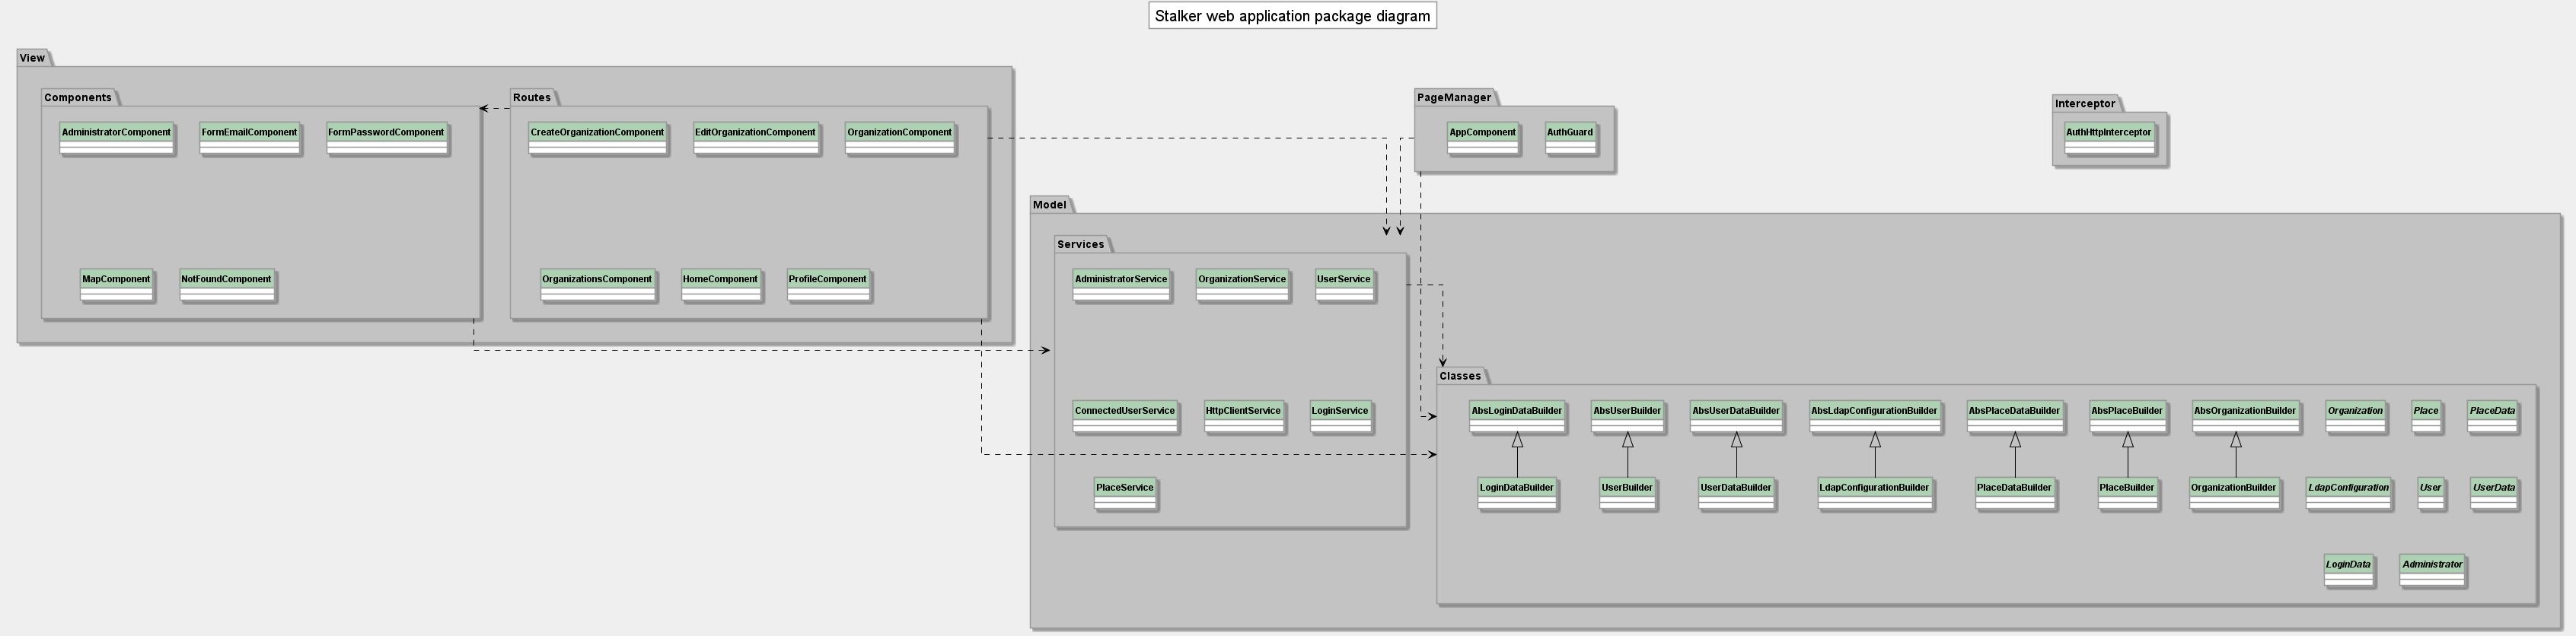
\includegraphics[width=6cm, height=22cm]{webapp-package-diagram.png}
  \caption{Diagramma dei package web application}%
  \label{fig:web-app-package-diagram}
\end{figure}

La web application di Stalker ha adottato il design pattern architetturale Model-View-ViewModel, come è possibile osservare in questo diagramma dei package il ViewModel è rappresentato dai \glossarioLocale{component} di angular si collegano ai propri template html che rappresentano invece la View, i \glossarioLocale{service} che gestiscono la business login e i modelli invece rappresentano il Model.
Questa architettura consente di lavorare in maniera asincrona nelle chiamate effettuate al server grazie agli \glossarioLocale{Observables}.
La vista inoltre rimane sempre aggiornata con il ViewModel tramite il \textit{two way data binding}.
\begin{figure}[H]
  \centering
  \scalegraphics{webapp-databinding.png}
  \caption{Two way data binding web application}%
  \label{fig:web-app-databinding}
\end{figure}

Tutti quanti i componenti e i servizi sono forniti dal provider di Angular, che prende i servizi e componenti dichiarati nel file \texttt{app.module.ts} e fa dependency injection dei suddetti ove fossero presenti come dipendenza.
In questo modo è presente una sola istanza per ogni servizio o componente in un dato momento dell'esecuzione.
% subs:architettura_generale (end)


\subsubsection{Comunicazione con il server}%
\label{subs:comunicazione_server}

La comunicazione con il server è lasciata completamente in mano ai servizi.
In Stalker è stato modellato un servizio per ogni dato che saremmo andati ad utilizzare, tutti questi servizi si interfacciano poi con il servizio HttpClientService che si occupa di mandare le richieste http rivolte agli endpoint definiti dalla nostra API e che vengono esposti dal server.
Tutte le richieste http in uscita vengono intercettate dalla class AuthHttpInterceptor che aggiunge un header per l'autenticazione in caso di chiamate agli endpoint di Stalker; il funzionamento di questa classe è definito nel dettaglio in §\ref{subs:autenticazione}.
Le risposte alle chiamate del server tornano poi ad HttpClientService che gestisce eventuali errori nella risposta lanciando un errore che provocherà un aggiornamento della vista da parte del component. In caso di una risposta positiva invece essa verrà restituita al servizio chiamante che dopo le opportune operazioni restituirà un Observable dell'oggetto richiesto dal component, che dopo aver effettuato una subscription all'oggetto possono aggiornare i propri campi dati.
A questo punto la vista si aggiornerà di conseguenza.

\begin{figure}[H]
  \centering
  \scalegraphics{webapp-http-calls-services.png}
  \caption{Servizi e chiamate http web application}%
  \label{fig:web-app-http-calls}
\end{figure}

Il seguente diagramma di sequenza illustra la serie di chiamate che intercorrono per visualizzare la pagina del profilo:
\begin{figure}[H]
  \centering
  \scalegraphics{webapp-http-call-sequence.png}
  \caption{diagramma di sequenza per visualizzare il profilo}%
  \label{fig:web-app-http-call-sequence}
\end{figure}

\subsubsection{Autenticazione e autorizzazione}%
\label{subs:autenticazione}

In Stalker l'autenticazione degli utenti viene gestita con i token JWT che identificano univocamente il permesso di un determinato utente di accedere all'applicazione web.
\begin{figure}[H]
  \centering
  \scalegraphics{webapp-auth.png}
  \caption{classi impegnate in autenticazione e autorizzazione}%
  \label{fig:web-app-auth}
\end{figure}
Il token di accesso viene creato dal server e poi arriva nell'header della risposta http alla web application, a questo punto la classe LoginService che aveva effettuato la richiesta di login conserva il token di accesso jwt in un cookie e il suo payload, ossia l'id dell'utente attuale, viene immagazzinato in \glossarioLocale{localstorage}.
Login service si occupa di ogni operazione che coinvolga l'accesso ad informazioni riguardanti l'autenticazione o l'autorizzazione come il logout o la verifica dei permessi dell'utente su una determinata organizzazione.
\begin{figure}[H]
  \centering
  \scalegraphics{webapp-loginservice.png}
  \caption{classe LoginService}%
  \label{fig:web-app-loginservice}
\end{figure}
Quest'ultima informazione in particolare è necessaria al corretto funzionamento della classe AuthGuard che si occupa di gestire l'accesso alle varie pagine della web application e il cui funzionamento è meglio descritto in §\ref{subs:navigazione}.
Dopo aver effettuato con successo il login ogni chiamata rivolta ad un endpoint di Stalker che richieda autenticazione verrà intercettata da AuthHttpInterceptor, che estende la classe di Angular \textit{HttpInterceptor}, e gli viene attaccato un nuovo header di autenticazione che ha come value il token JWT e che il server utilizzerà per autenticare la richiesta.
\begin{figure}[H]
  \centering
  \scalegraphics{webapp-authhttpinterceptor.png}
  \caption{classe AuthHttpInterceptor}%
  \label{fig:web-app-authhttpinterceptor}
\end{figure}
% subs:autenticazione (end)

\subsubsection{Navigazione}%
\label{subs:navigazione}

La navigazione nella web application di stalker è strettamente correlata all'autorizzazione poiché, essendo il target di questa applicazione amministratori di organizzazioni con diversi permessi, è indispensabile limitare l'accesso alle pagine per cui non si hanno i permessi.
Abbiamo deciso di sfruttare un meccanismo intrinseco di angular, le \glossarioLocale{Route Guard}, abbiamo dichiarato infatti la classe AuthGuard che ha come scopo il controllo dei permessi dell'utente e, qualora fossero sufficienti, permettere l'accesso alla pagina.
\begin{figure}[H]
  \centering
  \scalegraphics{webapp-authguard.png}
  \caption{Servizi e chiamate http web application}%
  \label{fig:web-app-authguard}
\end{figure}
I path soggetti a questo controllo sono stati identificati nel file \texttt{app.module.ts} con la seguente dichiarazione:
\begin{figure}[H]
  \centering
  \scalegraphics{webapp-appmodule-screen-1.png}
  \caption{app.module.ts screen}%
  \label{fig:web-app-appmodule-screen-1}
\end{figure}

Per alcuni path è stato inoltre dichiarato un campo data, che contiene in questo caso il ruolo necessario ad accedere al path.
\begin{figure}[H]
  \centering
  \scalegraphics{webapp-appmodule-screen-2.png}
  \caption{app.module.ts screen}%
  \label{fig:web-app-appmodule-screen-2}
\end{figure}
Abbiamo scelto di creare una guardia perché si integra automaticamente con Angular e risulta molto facile configurare i permessi necessari e le azioni da eseguire per ogni caso.
AuthGuard ha una dipendenza verso LoginService per ottenere le informazioni dell'utente.

% subs:navigazione (end)

\subsubsection{Rappresentazione dei modelli}%
\label{subs:modelli}

La web application di Stalker manipola principalmente due tipi di dati: utenti e organizzazioni.
\paragraph{User}%
\label{par:webapp/user}
\begin{figure}[H]
  \centering
  \scalegraphics{webapp-user.png}
  \caption{interfaccia User}%
  \label{fig:web-app-user}
\end{figure}
L'interfaccia User è costituito dall'Id univoco dell'utente e da due interfacce opzionali: UserData e LoginData.
La prima contiene i dati personali dell'utente e la sua Email ed è usata ad esempio nel profilo per visualizzare e modificare questi campi.
La seconda invece viene usata quando non sono necessarie le informazioni personali ma solo email e password, come nel caso dell'autenticazione.
% par:user (end)

\paragraph{Organization}%
\label{par:webapp/organization}
\begin{figure}[H]
  \centering
  \scalegraphics{webapp-organization.png}
  \caption{interfaccia Organization}%
  \label{fig:web-app-organization}
\end{figure}
L'interfaccia Organization possiede opzionalmente due interfacce: LdapConfiguration e un array di Place.
LdapConfiguration è presente solo se l'organizzazione è stata configurata come privata.
L'array di Place può essere vuoto se non vi sono luoghi in quell'organizzazione e può opzionalmente contenere un'interfaccia PlaceData che rappresenta i dati geografici del Place.
% par:organization (end)

\paragraph{Builder}%
\label{par:builder}
Le interfacce illustrate sopra sono state pensate per essere costruiti in modi diversi a seconda del loro scopo.
Abbiamo pensato quindi di deresponsabilizzare i component dall'onere di creare autonomamente queste interfacce che vengono quindi create attraverso Builder e che consentono anche di creare oggetti con dati che possono non essere presenti dall'inizio: come nel caso delle chiamate http al server Stalker.
\begin{figure}[H]
  \centering
  \scalegraphics{webapp-user-builder.png}
  \caption{User Builder}%
  \label{fig:web-app-user-builder}
\end{figure}
\begin{figure}[H]
  \centering
  \scalegraphics{webapp-organization-builder.png}
  \caption{Organization Builder}%
  \label{fig:web-app-organization-builder}
\end{figure}
% par:builder (end)

\paragraph{Estensione dei modelli}%
\label{par:estensione_interfacce_webapp}

L'utilizzo di builder per gestire la costruzione dei modelli rende molto facile estenderne o modificarne la rappresentazione.
Per estendere la rappresentazione di una di queste interfacce è sufficiente infatti implementare l'interfaccia estendendola o definirne un altra e creare un builder che estenda il builder astratto del tipo desiderato.

% par:estensione_interfacce_webapp (end)

% subs:modelli (end)

\subsubsection{Estensione}%
\label{subs:estensione_webapp}

Per estendere la web application con una nuova funzionalità è necessario:

\begin{itemize}
  \item creare tutti i component necessari a visualizzare e interagire con la nuova funzionalità.
  \item creare uno o più servizi che contengano la business logic della nuova funzionalità e che possono eventualmente dipendere da HttpClientService per l'invio di richieste al server o estendere quelli già esistenti.
  \item estendere le rappresentazioni dei modelli come descritto in~\ref{par:estensione_interfacce_webapp} se richiesto.
  \item dichiarare componenti e servizi aggiunti in \texttt{app.module.ts} al fine di renderli disponibili tramite dependency injection.
\end{itemize}
% subs:estensione-webapp (end)
% sub:architettura/web-app (end)
\end{document}
